\documentclass{report}

\usepackage[T2A]{fontenc}
\usepackage[utf8]{luainputenc}
\usepackage[english, russian]{babel}
\usepackage[pdftex]{hyperref}
\usepackage[14pt]{extsizes}
\usepackage{listings}
\usepackage{color}
\usepackage{geometry}
\usepackage{enumitem}
\usepackage{multirow}
\usepackage{graphicx}
\usepackage{indentfirst}

% Устанавливаю поля, отступы между абзацами, отступы в списке
\geometry{a4paper,top=2cm,bottom=3cm,left=2cm,right=1.5cm}
\setlength{\parskip}{0.5cm}
%\setlist{nolistsep, itemsep=0.3cm,parsep=0pt}

% Мой стиль для листинга кода
\lstset{language=C++,
		basicstyle=\footnotesize,
		keywordstyle=\color{blue}\ttfamily,
		stringstyle=\color{red}\ttfamily,
		commentstyle=\color{green}\ttfamily,
		morecomment=[l][\color{magenta}]{\#}, 
		tabsize=4,
		breaklines=true,
		breakatwhitespace=true,
  		title=\lstname,       
}

% Замена [1] -> 1. в списке литературы
\makeatletter
%\renewcommand\@biblabel[1]{#1.\hfil}
\makeatother

\begin{document}

% Титульный лист
\begin{titlepage}

\begin{center}
Министерство науки и высшего образования Российской Федерации
\end{center}

\begin{center}
Федеральное государственное автономное образовательное учреждение высшего образования \\
Национальный исследовательский Нижегородский государственный университет им. Н.И. Лобачевского
\end{center}

\begin{center}
Институт информационных технологий, математики и механики
\end{center}

\vspace{4em}

\begin{center}
\textbf{\LargeОтчет по лабораторной работе} \\
\end{center}
\begin{center}
\textbf{\Large«Умножение разреженных матриц.\\Элементы типа double.\\Формат хранения матрицы – столбцовый.»} \\
\end{center}

\vspace{4em}

\newbox{\lbox}
\savebox{\lbox}{\hbox{text}}
\newlength{\maxl}
\setlength{\maxl}{\wd\lbox}
\hfill\parbox{7cm}{
\hspace*{5cm}\hspace*{-5cm}\textbf{Выполнил:} \\ студент группы 381706-2 \\ Антипин А. С\\
\\
\hspace*{5cm}\hspace*{-5cm}\textbf{Проверил:}\\ доцент кафедры МОСТ, \\ кандидат технических наук \\ Сысоев А. В.
}

\vspace{\fill}

\begin{center} Нижний Новгород \\ 2020 \end{center}

\end{titlepage}
% Конец титульного листа

\setcounter{page}{2}

% Содержание
\tableofcontents
\newpage

% Введение
\begin{center}\section*{Введение}\end{center}
\addcontentsline{toc}{section}{Введение}
\par Разреженная матрица - это матрица с преимущественно нулевыми элементами. Если же большая часть элементов матрицы является ненулевыми, то матрица считается плотной. Разреженность данных определяется не количеством данных, а отношением занятых позиций  данных к количеству всех возможных позиций.
\par Хранение разреженной матрицы в памяти должно обеспечивать:
\begin{enumerate}
	\item экономию памяти,
	\begin{itemize}
		\item N*M – размерность матрицы
		\item Z – количество ненулевых элементов
		\item Z << N*M
	\end{itemize}
	\item быстрый доступ к нулевым и ненулевым элементам по их индексу.
\end{enumerate}
\par Реализация разреженных матриц связана со значительными издержками, и это делает их все более непрактичными по мере заполнении области данных значимыми величинами, и в тоже время, при большей разреженности эти структуры становятся более эффективными. Таким образом, cуществует хорошо определенный набор задач, для решения которых необходимо использовать  структуру данных типа разреженной матрицы. К таким задачам можно отнести, например:
\begin{enumerate} 
	\item численное решение больших разреженных систем уравнений,
	\item представление графов в виде разреженных матриц смежности для решения задач различного типа.
  \end{enumerate}
\newpage
% Конец введения

% Постановка задачи
\begin{center}\section*{Постановка задачи}\end{center}
\addcontentsline{toc}{section}{Постановка задачи}

\par В данной лабораторной работе необходимо выполнить следующие задачи:

\begin{enumerate} 

\item Написать структуру хранения разреженных матриц, включающую методы доступа к эдементам матрицы.
\item Реализовать последовательный алгоритм умножения двух разреженных матриц.
\item Реализовать параллельные варианты алгоритма умножения разреженных матриц с использованием различных технологий параллельных вычислений на системах с общей памятью, таких как OpenMP, Intel TBB и st::threads.
\item Доказать корректность полученных данных, провести замеры времени выполнения и сделать выводы из них.

\end{enumerate} 

\newpage
% Конец постановки задачи

% Описание алгоритма

\begin{center}\section*{Описание структуры хранения и алгоритма}\end{center}
\addcontentsline{toc}{section}{Описание структуры хранения и алгоритма}
\par \textbf{Разреженный столбцовый формат}, широко известен как CCS (Compressed Column Storage). Матрица хранится в виде трех массивов:
\begin{itemize} 
\item Массив значений \verb|Value| (построчно, сверху вниз);
\item Массив номеров строк \verb|Row|;
\item Массив индексов начала столбцов \verb|ColIndex|, где \verb|ColIndex[j]| указывает на начало j-го стоблца.
\end{itemize}
\par j-й столбец в массиве \verb|Value| находится по индексам от \verb|ColIndex[j]| до \\\verb|ColIndex[j + 1] – 1| включительно. Пустые столбцы обрабатываюся следующим образом - \verb|ColIndex[j] = ColIndex[j + 1]|.
Для последнего столбеца \verb|ColIndex[N+1] = Z|, где \verb|Z| - число элементов в матрице.
\par Пример:
\begin{figure}[htbp]
    \centering
    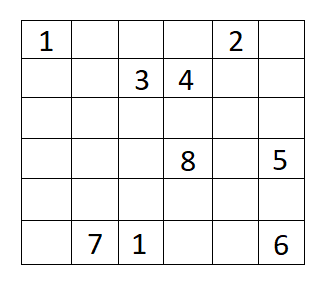
\includegraphics[width=0.3\textwidth]{../../../../modules/reports/antipin_a_sparse_matrix/example1.png}
    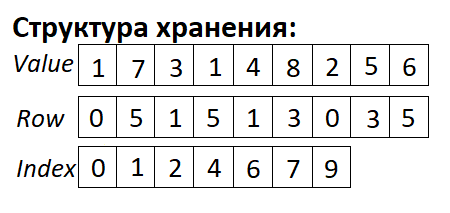
\includegraphics[width=0.3\textwidth]{../../../../modules/reports/antipin_a_sparse_matrix/example2.png}
    \caption{Пример разреженной матрицы и ее представления}\label{fig:../../../../modules/reports/antipin_a_sparse_matrix/example1.png}
\end{figure}

\par \textbf{Описание алгоритма умножения разреженных матриц:}
\begin{enumerate} 
	\item Проверка на совпадение размеров пришедших матриц;
	\item Транспонирование левой матрицы;
	\item Создание временного буфера на максимальное количество элементов в матрице размера N*N;
	\item Создание 2-ух циклов, один из которых вложен в другой (циклы от 0 до N);
	\item Перед созданием 3-его цикла выбирается где меньше элементов - в строке первой матрицы или в столбце второй;
	\item Перемножение элементов матриц, в цикле и получение нового элемента;
	\item Если элемент не нулевой, то он записывается в результирующую матрицу, в противном случае он отбрасывается;
	\item После завершения циклов, из буфера освобождаются все не занятые элементы.
\end{enumerate} 

Имплементацию данного алгоритма можно найти в приложении.

\newpage
% Конец описания

% Схема распараллеливания
\begin{center}\section*{Схема распараллеливания}\end{center}
\addcontentsline{toc}{section}{Схема распараллеливания}
\par Так как формировани отдельных столбцов результирующей матрицы не зависит друг от друга, то можно распараллелить внешний цикл, который как раз и отвечает за их формирование. При этом буфер будет отдельным для каждого столбца (вектор векторов).
\subsection*{OpenMP}
\addcontentsline{toc}{subsection}{OpenMP}
\par Воспользуемся встроенной директивой \verb|#pragma omp parallel for|, которая отвечает за распараллеливание циклов. Внутренней содержание цикла осталось почти без изменений. В конце функции выполнено объединение получившихся буферов в результирующих матрицу (каждый из них оказывается почти пустым).

\subsection*{TBB}
\addcontentsline{toc}{subsection}{TBB}
\par В фунции инициализирем параллельную секцию с помощью метода \\\verb|tbb::task_scheduler_init init()|, куда передается количество потоков. Далее воспользуемся функцией \verb|tbb::parallel_for()|, в которую передается интервал цикла и лямбда функция, в которую помещается внутреннее содержание цикла. После выполняется объединение в результирующую матрицу получившихся столбцов.

\subsection*{std::threads}
\addcontentsline{toc}{subsection}{Std::threads}
\par В цикле создаем необходимое число потоков, в каждый из которых передается фунцкия с нужным интервалом внешенго цикла, внутреннее содержание цикла остается неизменным. Далее в другом цикле ожидется завершение всех потоков и их удаление. Затем происходит объединение буфера в результирующую матрицу.

\newpage
% Конец схемы распараллеливания

% Эксперименты
\begin{center}\section*{Эксперименты}\end{center}
\addcontentsline{toc}{section}{Эксперименты}
Конфигурация системы:
\begin{itemize}
\item Процессор: AMD Ryzen 5 3600, 6 Cores, 12 Threads, 3.6-4.2 GHz;
\item Оперативная память: 16Gb DDR4 2766 MHz;
\item ОС: Windows 10 Pro 64bit;
\end{itemize}

\par Для проверки корректности выполнения программ были написаны \verb|Google Tests|, которые проверили как саму структуру хранения, так и алгоритм умножения матриц. Для тестирования производительности программ, написанных на основе разных технологий, были произведены замеры их времени работы на разном количестве исходных данных. Далее приведена таблица со средними результатами экспериментов (5 прогонов). В левой колонке размерность матрицы N, в остальных время работы в секундах. Важно отметить, что во всех тестах коэфиициент разреженности матрици был 500 (т.е. всего ненулевых элементов было \verb|N*N/500|).

\begin{tabular}{ | l | l | l | l | l | }
	\hline
	\verb|Кол-во элем.| & \verb|Посл. алг.| & \verb|OpenMP| & \verb|TBB| & \verb|std::threads| \\ \hline
	500 & 0.009 & 0.003 & 0.002 & 0.003 \\
	1000 & 0.062 & 0.010 & 0.011 & 0.11 \\
	5000 & 1.568 & 0.474 & 0.497 & 0.511 \\
	10000 & 18.925 & 4.088 & 4.484 & 4.585 \\
	15000 & 68.786 & 15.031 & 18.861 & 19.476 \\
	\hline
\end{tabular}
\par По результатам экспериметов видно, что самой быстрой оказалась реализация, основанная на OpenMP, за ней TBB и с небольшим отставанием std::threads. Вероятнее всего TBB оказалась медленне из-за тестирования на процессоре от AMD, а также потому что не использовался встроенный в него планировщик задач. Тем не менее, прирост скорости работы от OpenMP реализации оказался примерно 4.5 раза, что является достаточно существенным.
 
\newpage
% Конец результатов экспериментов

% Заключение
\begin{center}\section*{Заключение}\end{center}
\addcontentsline{toc}{section}{Заключение}

По результатам лабораторной работы были выполнены следующие задачи:

\begin{enumerate} 
\item Написана структура хранения разреженных матриц;
\item Написан последовательный алгоритм умножения разреженных матриц, произведены замеры времени его выполнения;
\item Реализованы параллельные варианты алгоритма умножения разреженных матриц с использованием различных технологий, таких как OpenMP, TBB и std::threads, и также произведены замеры их времени работы.
\item Все методы были также проверены на корректность с помощью Google Tests.
\end{enumerate} 

\newpage
% Конец заключения

% Список литературы
\begin{thebibliography}{1}
\addcontentsline{toc}{section}{Литература}

\bibitem{Gergel} Гергель В.П., Стронгин Р.Г. Основы параллельных вычислений для многопроцессорных вычислительных систем. Учебное пособие – Нижний Новгород: Изд-во ННГУ им. Н.И. Лобачевского, 2003. 184 с. ISBN 5-85746-602-4.

\bibitem{Barkalov} Баркалов К.А. Параллельные численные методы. Решение разреженных СЛАУ. Н. Новгород: Изд-во Нижегородского госуниверситета им. Н.И. Лобачевского, 2011

\bibitem{Wiki1} Wikipedia: the free encyclopedia [Электронный ресурс] // URL: https://ru.wikipedia.org/wiki/\verb|Разреженная_матрица| (дата обращения: 17.03.2020)

\bibitem{Wiki2} qwe.wiki [Электронный ресурс] // URL: https://ru.qwe.wiki/wiki/\verb|Sparse_matrix| (дата обращения: 17.03.2020)

\end{thebibliography}
\newpage
% Конец списка литературы

% Приложение
\begin{center}\section*{Приложение}\end{center}
\addcontentsline{toc}{section}{Приложение}
Код:

\lstinputlisting[language=C++]{../../../../modules/task_1/antipin_a_matrix_multiplication/matrix_multiplication.h}
\lstinputlisting[language=C++]{../../../../modules/task_1/antipin_a_matrix_multiplication/matrix_multiplication.cpp}
\lstinputlisting[language=C++]{../../../../modules/task_1/antipin_a_matrix_multiplication/main.cpp}

\lstinputlisting[language=C++]{../../../../modules/task_2/antipin_a_matrix_multiplication/matrix_multiplication.h}
\lstinputlisting[language=C++]{../../../../modules/task_2/antipin_a_matrix_multiplication/matrix_multiplication.cpp}
\lstinputlisting[language=C++]{../../../../modules/task_2/antipin_a_matrix_multiplication/main.cpp}

\lstinputlisting[language=C++]{../../../../modules/task_3/antipin_a_matrix_multiplication_tbb/matrix_multiplication.h}
\lstinputlisting[language=C++]{../../../../modules/task_3/antipin_a_matrix_multiplication_tbb/matrix_multiplication.cpp}
\lstinputlisting[language=C++]{../../../../modules/task_3/antipin_a_matrix_multiplication_tbb/main.cpp}

\lstinputlisting[language=C++]{../../../../modules/task_4/antipin_a_matrix_multiplication_std/matrix_multiplication.h}
\lstinputlisting[language=C++]{../../../../modules/task_4/antipin_a_matrix_multiplication_std/matrix_multiplication.cpp}
\lstinputlisting[language=C++]{../../../../modules/task_4/antipin_a_matrix_multiplication_std/main.cpp}

\end{document}